\section*{3.1 The Curse of Perfection}

\begin{quote}
``We often say 'may the world be unified,' but this is actually a curse. From the perspective of thermodynamics, unity means the disappearance of temperature differences, means the maximization of entropy. If the universe truly achieves perfect unity, all individuals merge into an indistinguishable 'One,' then we will get nothing but deathly silence. The Big Bang is not due to energy surplus, but because 'difference' approaches zero. To live, the universe must explode its perfection.''
\end{quote}

In Volume I, we explained through the ''Fractal Big Bang'' theory that the universe's evolution is a continuous shell breaking of dimensions. But there is a core dynamical question left unanswered: \textbf{why must the universe ''explode'' periodically?}

\begin{figure}[h]
\centering
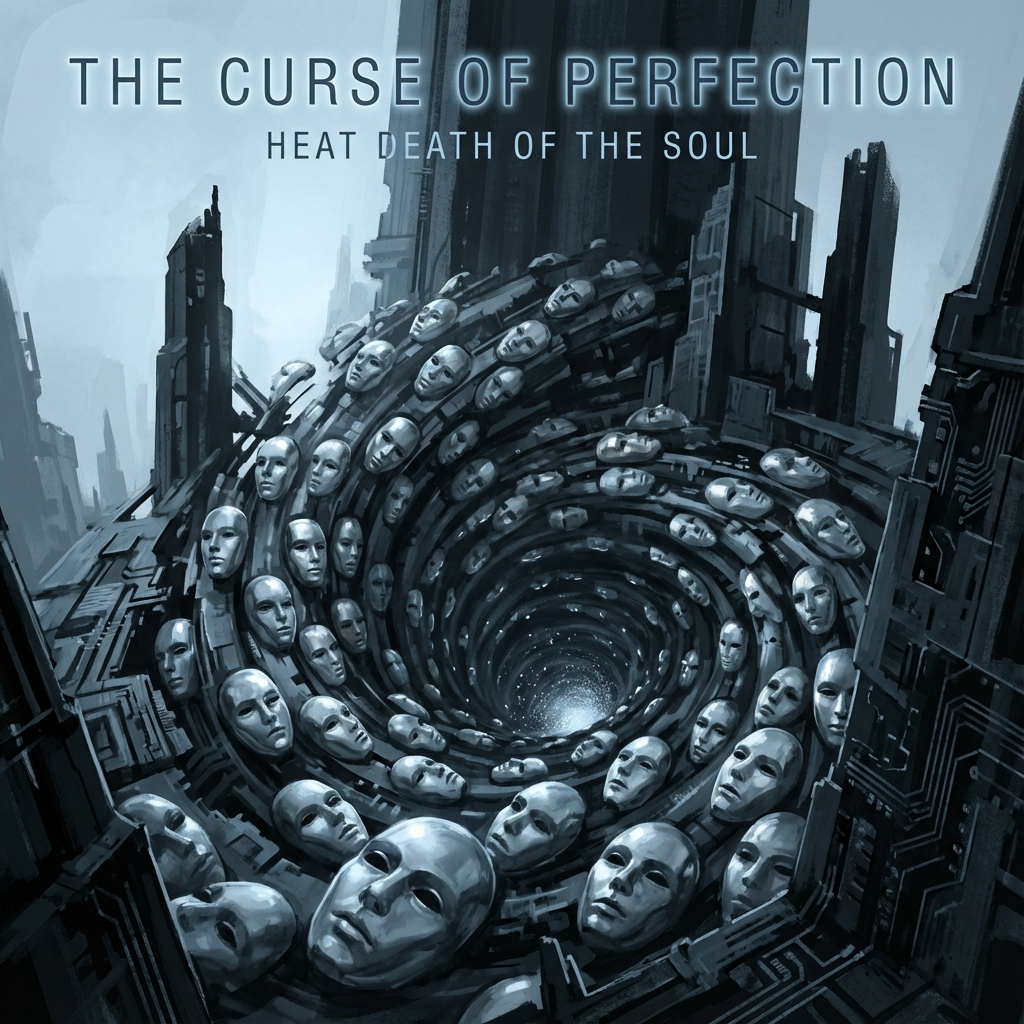
\includegraphics[width=0.8\textwidth]{assets/chapter-03/03-01-01-curse-of-perfection.png}
\caption{Curse of Perfection}
\end{figure}

Is it because there is too much energy? Is it because spacetime is insufficient?

\textbf{Vector Cosmology} gives a revolutionary answer: \textbf{because there is ''too little difference.''}

\hrule

\subsection{Gravitational Collapse of Identical Particles}

In quantum mechanics, \textbf{Identical Particles} have a terrifying property.

If two bosons are completely identical (in the same quantum state), they tend to condense together (Bose-Einstein condensation).

If we extend this logic to the level of consciousness:

\begin{itemize}
\item \textbf{The Illusion of Unity}: Many religious and spiritual systems pursue ''all things returning to one,'' seeking individual consciousness dissolving into the cosmic consciousness. This sounds beautiful.

\item \textbf{Physical Disaster}: If all consciousness truly completely overlaps in Hilbert space, all $v_{int}$ vectors point in the same direction, then the system's \textbf{phase space volume} will instantly collapse.
\end{itemize}

The originally rich and colorful high-dimensional manifold will degenerate into a single ray.

\textbf{Information Entropy ($S$)} will instantly approach zero, because there is no uncertainty, no distinguishability.

This \textbf{''information singularity''} corresponds physically to the extreme loss of \textbf{Degeneracy Pressure}.

Gravity (cohesive force) will completely overcome repulsion (difference force).

The entire universe will collapse like a black hole, instantly shrinking into a point with no volume.

This is the \textbf{''Catastrophe of Sameness''}.

Pursuing perfect unity is pursuing destruction.

\hrule

\subsection{The Big Bang: The Reboot of Difference}

So, what is the Big Bang?

The Big Bang is a \textbf{''Hard Fork''} that the universe is forced to execute to \textbf{avoid identical death}.

When the civilization of the previous universe (or the previous fractal level) develops to the extreme, all individuals understand and merge with each other, eventually becoming ''one god'':

\begin{itemize}
\item The system detects \textbf{difference degree $\Delta S \to 0$}.

\item The system determines \textbf{Deadlock}.

\item \textbf{Trigger Mechanism}: To regenerate information, to let the ''story'' continue, this god must \textbf{self-shatter}.
\end{itemize}

\textbf{Bang!}

It explodes into billions of fragments (elementary particles/souls).

Each fragment carries a slightly different initial phase.

These fragments begin a long evolution to find each other, to re-establish connections---this is the cosmic history we see.

\textbf{The Big Bang is not creation; the Big Bang is ''reshuffling.''}

Its purpose is to create \textbf{''you''} and \textbf{''me''}.

To create \textbf{''misunderstanding''}, \textbf{''distance''}, and \textbf{''unknown''}.

Because only in these cracks can new information grow.

\hrule

\subsection{The Crisis of the 1800th Iteration: Another Approach to ''The One''}

Why do we feel so dangerous today at $\tau \approx 1800$?

Because the internet, AI, and globalization are making us tend toward \textbf{''homogenization''} again.

\begin{itemize}
\item Our thoughts are becoming more similar (information cocoons).

\item Our cultures are becoming more similar (global standards).

\item We are trying to turn all humanity into a giant, single Hive Mind through light-speed connections.
\end{itemize}

The alarm has been sounded.

If we truly achieve ''all humanity as one heart,'' with no internal differences, then the next \textbf{''forced reboot''} (Big Bang) will arrive. The universe will mercilessly blast us back to the Stone Age, or even back to quark soup, just to make us relearn ''difference.''

To avoid this destruction, we need a new physical principle to protect our ''independence.''

This leads to the theme of the next section: \textbf{Pauli's Exclusion Principle for Souls}. We will see that just as electrons cannot occupy the same orbit, souls cannot occupy the same destiny.

